\chapter{Cómputo con Python}
\graphicspath{{img/herramientas/}}

El objetivo de este capítulo lo podríamos resumir en aprender lo básico para ``hacer que los computadores trabajen para nosotros'', es decir, aprender a usar unas herramientas básicas que nos permitan facilitar tareas que de otro modo serían tediosas y en las que se podrían cometer errores fácilmente. Este capítulo no pretende ser un tutorial sobre el manejo de Python para Ingeniería, para ello se sugiere las \emph{notas de clase} ``SciPy Lecture notes'' \cite{scipy-lectures} o el libro \cite{book:programming_computations}.

\section{Convenciones para archivos}

Con el fin de eliminar conflictos a la hora de manipular archivos o compartirlos, se recomienda tener en cuenta las siguientes convenciones en los nombres
de archivos y carpetas (también llamados directorios) -que en esencial son archivos-:

\begin{itemize}
    \item Use letras minúsculas: Windows y Mac no diferencian capitalización del texto en los nombres de archivos y a raíz de ello, Dropbox
    tampoco (sin importar si es usado Linux-). Mantener la convención de minúsculas evitará posibles conflictos de archivos y
    que todos los colaboradores tengan los archivos con los mismos nombres (Dropbox no actualiza el cambio de capitalización en el nombre de los archivos)
    para que los llamados de archivos funcionen adecuadamente. Ejemplo: es preferible \texttt{trabajo.txt} que \texttt{Trabajo.txt}.
    \item Use guion bajo en lugar de espacio: Si por motivos de legibilidad requiere un espacio en el nombre del archivo, reemplace este por un guion bajo.
    Ejemplo: es preferible \texttt{trabajo\_Python.zip} que \texttt{trabajo Python}.
    \item No use letras acentuadas: Las letras con acentos difieren en su representación según la codificación usada pero la mayor parte de codificaciones
    se basan en extender ASCII-7, así las letras sin acentos (alfabeto inglés particularmente) no presentarán problemas. Ejemplo: es preferible \texttt{analisis.py}
    que \texttt{análisis.py}.
    \item No use símbolos de puntuación o caracteres especiales: La mayor parte de estos símbolos poseen significados por lo cual podrían ser omitidos o interpretados
    erróneamente. Un punto al inicio del nombre de una archivo en Unix representa un archivo invisible, una virgulilla (\texttt{~}) suele presentarse en nombres
    que corresponden a copias de seguridad o archivos temporales, los paréntesis se usan con números para indicar archivos duplicados. Su uso con invocación de comandos
    puede llevar a resultados no esperados, como el caso del asterisco (\texttt{*}) que se interpreta como un comodín en el nombre (equivale a cualquier combinación de caracteres). 
\end{itemize}

Así, dejaremos como regla que los nombres de archivos y carpetas solo serán formados por caracteres alfanuméricos no acentuados en minúscula y guiones bajos.
Esta misma convención (salvo por la posibilidad de usar mayúsculas) aplica como regla en los nombres de las variables a la hora de programar (con excepción
de algunos lenguajes como Python3 y Julia, que al soportar la codificación UTF-8 no tienen problema con caracteres especiales y acentos).

\section{Python}

Python es un lenguaje de programación multiplataforma (soporta Windows,
Linux, Mac e incluso existen versiones para móvil) orientado a objetos e
interpretado (el código ejecutable no es optimizado para la máquina en
cuestión y siempre requiere del código fuente para su uso). Es un
lenguaje con una gran comunidad usandolo en diversas disciplinas lo cual
facilita encontrar muchos paquetes útiles para diferentes labores, entre
ellas la modelación computacional, y una base/núcleo del lenguaje listo
para muchas tareas (sin requerir instalaciones adicionales existen
múltiples utilidades que no son básicas, como el manejo de bases de
datos SQLite, solicitudes web, análisis semántico de HTML, protocolos de
correo e interfaces gráficas con TK).

Al día de hoy la última versión liberada de Python es la 3.7.0 pero
recomendamos para el uso de la versión 3.6.5 e instalarlo usando la
distribución de Python Anaconda.

\subsection{Tipos de datos y operaciones}

Los tipos de datos básicos que encontramos en Python3 son numéricos,
lógicos y cadenas de caracteres. Aparte de estos, podemos destacar la
existencia de los contenedores que permiten la agrupación de datos
(incluso de diverso tipo) en una misma variable. Es importante tener en
cuenta que la asignación en variables es necesaria para la reutilización
de sus valores en partes posteriores de un código y ayuda a la
legibilidad del mismo. Igualmente, para todos los tipos de variables,
podemos realizar la impresión del valor por medio de la función interna
\texttt{print} (la cual usaremos para ver los resultados de nuestras
manipulaciones, pero no es necesaria en una consola interactiva como
\emph{Jupyter}).

\begin{listing}[H]
    \begin{minted}[mathescape, gobble=8, frame=lines,
                framesep=2mm]{python}
        a = 5 # Asignación
        print(a) # Imprime a salida estándar. Conversión implícita.
    \end{minted}
\end{listing}

Los tipos de datos numéricos pueden ser enteros o flotantes (el
equivalente de los reales) y en unión al sufijo \texttt{j}, la
construcción de imaginarios y complejos es posible. Python da soporte de
las operaciones aritméticas para datos numéricos, teniendo presente que
la operación de potencia se usa con \texttt{**}, una raíz es lo mismo
que una potencia al inverso del índice de la raíz y el operador módulo
es \texttt{\%}.

\begin{listing}[H]
    \begin{minted}[mathescape, gobble=8, frame=lines,
                framesep=2mm]{python}
        print(2 + 3) # Suma: debe imprimir 5
        print(2.3 * 4) # Producto: debe imprimir 9.2
        print(9/4) # División: debe imprimir 2.25
        print(3 - 1.5) # Resta: debe imprimir 1.5
        print(1.1**2) # Potenciación: debe imprimir 1.21
        print(4**0.5) # Raíz: imprime 2.0 (potencia 0.5 es raíz cuadrada)
        print(5%2) # Módulo (residuo): debe imprimir 1
        print(1-7j) # Número complejo
        print(4 - 2j + 6j) # Operaciones complejos: 4 + 4j
    \end{minted}
\end{listing}


Los valores lógicos correspondientes al álgebra booleana y las tablas de
verdad, verdadero y falso, se usan en Python como \texttt{True} y
\texttt{False} respectivamente. Dado que Python distingue entre
mayúsculas y minúsculas, es importante notar la mayúscula inicial de los
valores lógicos. Internamente distintos tipos de datos poseen
equivalencias a los valores lógicos para permitir ahorrar pasos de
conversión, como por ejemplo los datos numéricos son equivalentes a
\texttt{True} siempre que el valor sea distinto de cero, y si es cero
equivale a \texttt{False}. En las cadenas de caracteres, es
\texttt{True} cualquier cadena que tenga al menos un carácter.

\begin{listing}[H]
    \begin{minted}[mathescape, gobble=8, frame=lines,
                framesep=2mm]{python}
        print(True or False) # disyunción: debe imprimir True.
        print(True and False) # conjunción: debe imprimir False.
        print(not(True)) # negación: debe imprimir False.
    \end{minted}
\end{listing}


Finalmente, las cadenas de caracteres son en si mismos contenedores,
pero no se distingue entre carácter y cadena de caracteres como sucede
en otros lenguajes (\emph{char} y \emph{string}). Al ser este un
contenedor se puede hablar de elementos que le pertenecen y en
particular, este es un contenedor ordenado, por lo cual es posible
hablar de posiciones en él. Una cadena de caracteres es delimitada por
comillas simples (\texttt{'}) o altas (\texttt{"}).

En las cadenas de caracteres, la manipulación que se realiza es
principalmente recurriendo a métodos de la clase \texttt{string}
(orientación a objetos), pero se pueden usar algunos operadores y
funciones internas (\emph{built-in}) para manipulaciones frecuentes como
la concatenación, repetición y longitud.

\begin{listing}[H]
    \begin{minted}[mathescape, gobble=8, frame=lines,
                framesep=2mm]{python}
        texto1 = 'Hola' 
        texto2 = "mundo"
        texto_concatenado = texto1 + " " + texto2 
        print(texto_concatenado)
        print(texto_concatenado * 5) 
        print(len(texto_concatenado))
        print(texto1[2]) 
    \end{minted}
\end{listing}


A parte de las cadenas de caracteres, hay otros contenedores definidos
en el lenguaje Python que son listas, tuples, conjuntos y diccionarios.
Las listas y los tuples poseen índices, los conjuntos no son ordenados y
no permiten elementos duplicados, los diccionarios asocian claves y
valores a las mismas, los tuples son inmutables (una vez definidos no se
puede cambiar su valor). Para mayor claridad, siempre se recomienda
manipular los contenedores accediendo a los métodos definidos en sus
clases, esto se con un \texttt{.} (punto) después de la variable seguida
del nombre del método. Todos los contenedores definen una longitud que
puede ser accedida con la función interna \texttt{len}.

A continuación se ejemplifican manipulaciones sobre los contenedores.

\begin{listing}[H]
    \begin{minted}[mathescape, gobble=8, frame=lines,
                framesep=2mm]{python}
        lista_ej = [1, 2, 3]
        print(lista_ej)
        lista_ej.append(5)
        print(lista_ej)
        lista_ej.extend([7, 9])
        print(lista_ej)
        print(lista_ej[0])
        print(lista_ej[-1])
        print(lista_ej[1:3])
        lista_ej.insert(2, 10) 
        print(lista_ej)
    \end{minted}
\end{listing}


Las posibilidades con tuples se ilustran en su totalidad en el siguiente
bloque de código. No hay más métodos disponibles que los ilustrados.

\begin{listing}[H]
    \begin{minted}[mathescape, gobble=8, frame=lines,
                framesep=2mm]{python}
            tuple_ej = (3, 4, 5, 3)
            print(tuple_ej)
            print(tuple_ej[1])
            print(tuple_ej.count(3))
            print(tuple_ej.index(3))
    \end{minted}
\end{listing}


\begin{listing}[H]
    \begin{minted}[mathescape, gobble=8, frame=lines,
                framesep=2mm]{python}
        diccionario_ej = {"lenguaje": "python", "version": 3} 
        print(diccionario_ej) # Imprime diccionario original
        print(diccionario_ej.get("lenguaje")) 
        print(diccionario_ej["lenguaje"])
        diccionario_ej.update({"tipo": "interpretado"}) 
        print(diccionario_ej) 
    \end{minted}
\end{listing}


En general los tipos de datos que son contenedores, se les puede aplicar
operadores de pertenencia como en la teoría de conjuntos. Estos son
\texttt{in} para saber si el elemento pertenece y \texttt{not\ in} para
saber si el elemento no pertenece.

\begin{listing}[H]
    \begin{minted}[mathescape, gobble=8, frame=lines,
                framesep=2mm]{python}
        # Lista de planetas del sistema solar
        planetas = ["Mercurio", "Venus", "Tierra", "Marte", \
            "Júpiter", "Saturno", "Urano", "Neptuno"]
        print("Venus" in planetas) 
        print("Plutón" in planetas) 
        print("Tierra" not in planetas)
        print("Vulcano" not in planetas)
    \end{minted}
\end{listing}

Para operaciones más elaboradas de la teoría de conjuntos, se puede usar
el contenedor de conjuntos.

\begin{listing}[H]
    \begin{minted}[mathescape, gobble=8, frame=lines,
                framesep=2mm]{python}
        conjunto_ej1 = {1, 2, 3, 1} 
        print(conjunto_ej1) 
        conjunto_ej2 = {2, 6, 1}
        print(conjunto_ej1.union(conjunto_ej2))
        print(conjunto_ej1.intersection(conjunto_ej2)) 
        print(conjunto_ej1.difference(conjunto_ej2)) 
    \end{minted}
\end{listing}

También se definen los operadores relacionales, y su comportamiento
depende del tipo de dato. En los valores numéricos es acorde a su
posición en la recta numérica (enteros y flotantes), en las cadenas de
caracteres es según el orden alfabético y en los demás contenedores es
según su longitud.

\begin{listing}[H]
    \begin{minted}[mathescape, gobble=8, frame=lines,
                framesep=2mm]{python}
        print(5 < 10)
        print(7 >= 7)
        print(6 != 5) # Operador "es diferente"
        print("zapato" > "esternocleidomastoideo")
        print("ojo" <= "hoja")
        print([1, 2] > [5, 6, 7])
        print([1, 0] == [1, 0])
    \end{minted}
\end{listing}


El operador de igualdad o las desigualdades flexibles, considerar la
igualdad bajo la coincidencia del valor. Esta aclaración es importante
en los contenedores donde las desigualdades estrictas se basan en la
longitud (igual longitud no es igual el elemento).

\subsection{Estructuras de control}

Las estructuras de control son los elementos que guían el flujo de datos
a través del código. Esencialmente se pueden mencionar las estructuras
condicionales, cíclicas y manejados de errores. Las estructuras de
control permiten crear acciones según valores lógicos generados por
expresiones cuya salida sea de tipo lógico (se recomienda para esta
parte tener muy presente los operadores lógicos, relacionales y de
pertenencia).

Es importante aquí, recalcar que las estructuras requieren el uso de
sangría para determinar cuando se entra o se sale de la misma. La línea
que abre la estructura termina con \texttt{:} y las siguientes se
sangran a 4 espacios (se recomienda configurar el editor de código para
convertir una tabulación en 4 espacios). Para salir de la estructura se
remueve el sangrado.

Las estructuras condicionales realizan validación de una condición (o
secuencia de condiciones) una sola vez, y según la primera que ocurra se
realiza la ejecución de las sentencias presentes en su bloque. En
Python, tenemos solo la estructura \texttt{if\ ...\ elif\ ...\ else}. La
única parte obligatoria de la estructura es \texttt{if} para evaluar la
expresión lógica, y en caso de ser verdadera ejecutar sus sentencias. Si
se desea agregar condiciones adicionales, usamos \texttt{elif} de la
misma forma, con la expresión lógica a su lado. Finalmente, usamos
\texttt{else} para establecer una ejecución por defecto cuando las
condiciones revisadas no se cumplen.

\begin{listing}[H]
    \begin{minted}[mathescape, gobble=8, frame=lines,
                framesep=2mm]{python}
        nota = 3.5
        if (nota < 0) or (nota > 5):
            print("Nota inválida")
        elif nota < 3:
            print("Nota perdida")
        else: # Caso sobrante
            print("Nota ganada")
    \end{minted}
\end{listing}


En las estructuras cíclicas podemos encontrar los ciclos \texttt{while}
(mientras) y \texttt{for} (para). En el primero la repetición de un
bloque de sentencias se da si la evaluación de una expresión lógica es
verdadera. En el caso de la segunda, es un caso particular donde la
expresión es de pertenencia (se recorren todos los elementos
pertenecientes al contenedor dispuesto).

\begin{listing}[H]
    \begin{minted}[mathescape, gobble=8, frame=lines,
                framesep=2mm]{python}
        cont = 2
        while cont < 21:
            print(cont)
            cont = cont**2
    \end{minted}
\end{listing}


\begin{listing}[H]
    \begin{minted}[mathescape, gobble=8, frame=lines,
                framesep=2mm]{python}
        for numero in range(10):
            print("Ojala Bart supiera programar.")
    \end{minted}
\end{listing}


En el ciclo \texttt{for} del ejemplo vemos un generador, \texttt{range},
que es equivalente a un contenedor cuya única función es recorrer sus
elementos. Es una forma eficiente de crear contenedores de números que
siguen una secuencia. El argumento de \texttt{range} es una unidad
superior al límite superior deseado (en general, se está creando un
intervalo semiabierto a la derecha).

Finalmente la estructura de manejo de errores permite hacer captura de
errores durante la ejecución para evitar una finalización esperada de la
ejecución. Cuando ocurren errores en la ejecución, esta termina a menos
que se capture el error y de paso es posible hacer un manejo del mismo
(como darle una advertencia al usuario o hacer un procedimiento
alternativo).

\begin{listing}[H]
    \begin{minted}[mathescape, gobble=8, frame=lines,
                framesep=2mm]{python}
        dividendo = 10
        divisor = 0
        try:
            cociente = dividendo / divisor
        except:
            print("Solo Chuck Norris puede dividir por cero.")
    \end{minted}
\end{listing}


\subsection{Funciones y módulos}

Podemos definir funciones para facilitar la legibilidad y reutilización
de código cuando tenemos líneas de código recurrentes en el programa.
Por ejemplo, en un mismo programa se calcula varias veces la altura de
una caída libre y ello implica usar la misma forma de líneas (solo
cambiando variables o números), así que podemos hacer una función para
ello.

Las funciones requieren iniciar la línea con \texttt{def} para indicar
que se definirá una función. A continuación sigue el nombre que daremos
a la función y finalmente paréntesis. Dentro de los paréntesis van los
argumentos de la función separados por coma (si no requiere argumentos
se deja vacío el paréntesis).

Hay varios tipos de argumentos: obligatorios que van al inicio,
opcionales que poseen indicación de su valor por defecto en caso de
estar ausentes (se acompañan de la asignación), argumentos opcionales
sin valor por defecto (\texttt{*args}) y argumentos opcionales con clave
(\texttt{**kwargs}).

\begin{listing}[H]
    \begin{minted}[mathescape, gobble=8, frame=lines,
                framesep=2mm]{python}
        def altura_caida(t, g=9.76): 
            return 0.5 * g * t**2
    \end{minted}
\end{listing}

\begin{listing}[H]
    \begin{minted}[mathescape, gobble=8, frame=lines,
                framesep=2mm]{python}
        print(altura_caida(2)) 
        print(altura_caida(2, 10)) 
    \end{minted}
\end{listing}


Se pueden crear módulos para compartir nuestras funciones, clases y
constantes en un archivo o para permitir su reutilización de una manera
más simple. Para ello es necesario guardar estas definiciones en un
archivo \texttt{.py}, donde el nombre del archivo será el nombre del
módulo y por ende el nombre usado para su invocación.

Existen tres formas para realizar los llamados a las definiciones en los
módulos, y se ilustraran con módulos existentes en el núcleo de Python:

Se puede importar el nombre de la función de manera explícita desde el
módulo que la contiene. Para hacer uso de la función se llama
directamente con su nombre.

\begin{listing}[H]
    \begin{minted}[mathescape, gobble=8, frame=lines,
                framesep=2mm]{python}
        from math import sqrt
        print(sqrt(4))
    \end{minted}
\end{listing}

Se puede importar el módulo y posteriormente invocar la función desde el
espacio de nombres del módulo, usando el nombre del módulo seguido de
punto y el nombre de la función.

\begin{listing}[H]
    \begin{minted}[mathescape, gobble=8, frame=lines,
                framesep=2mm]{python}
        import random
        print(random.randint(2, 15))
    \end{minted}
\end{listing}

Finalmente se puede importar todos los elementos visibles en un módulo y
que estos se accedan directamente con su nombre. Esta forma no es
recomendable por posibles colisiones de nombre (si el mismo nombre es
importado desde distintos módulos) y hacer la revisión de código es
compleja al no saber la procedencia de la función.

\begin{listing}[H]
    \begin{minted}[mathescape, gobble=8, frame=lines,
                framesep=2mm]{python}
        from os import * 
        print(listdir())
    \end{minted}
\end{listing}



\subsection{Actividad}

\begin{enumerate}
\def\labelenumi{\arabic{enumi}.}

\item
  ¿Cuál es la diferencia entre los números flotantes y los números
  reales?
\item
  Realice un código en Python que permita ilustrar la diferencia de
  operar números flotantes respecto a números reales.
\item
  Realice un código en Python que determine el número de veces que se
  repite el carácter `a' en el nombre de su docente.
\item
  Realice una función que reciba un número complejo y determine su
  módulo.
\item
  Realice una función que determine el área de un triángulo dadas las
  longitudes de sus lados.
\item
  Realice una rutina que imprima la tabla de verdad correspondiente a
  \(\neg(\neg A \wedge B) \vee C\), calculando el valor de verdad final
  con los operadores lógicos. Debe tener adecuada alineación la tabla.
\item
  Realice de dos maneras diferentes un código que le ayude a hacer una
  plana de 5000 repeticiones que digan ``Yo voy a ganar la materia.''.
  Debe ser repetición por línea.
\item
  Elabore una función para determinar si un producto dado se encuentra
  en la lista de mercado. La función debe recibir como primer argumento
  una lista de cadena de caracteres cuyos elementos son los productos a
  comprar y el segundo argumento es una cadena de caracteres que
  representa el producto que deseamos consultar si fue incluido. La
  función debe retornar ``Incluido'' si ya estaba en la lista y
  ``Falta'' si no lo está.
\item
  Realice un diccionario donde el campo de clave corresponda a un número
  y el campo de valor al nombre de alguien (ingrese al menos 3
  elementos). Realice ahora una función que al recibir como primer
  argumento un diccionario y segundo argumento un número, retorne el
  nombre del individuo si existe el número y retorne ``ausente'' si no
  está el número.
\item
  Desarrolle un módulo \texttt{geometria} con funciones para el cálculo
  del área de al menos dos geometrías planas y del volumen de dos
  sólidos. Luego, desde la consola importe el módulo y haga uso de las
  funciones definidas.
\end{enumerate}


\subsection{Recursos adicionales}

Para complementar el aprendizaje de Python y su instalación, se
recomiendas las siguientes fuentes:

\begin{itemize}
\item
  \href{https://docs.anaconda.com/anaconda/install/}{Anaconda Python}.
\item
  \href{https://github.com/saint-germain/Python3Espanol}{Curso de
  introducción a Python3}.
\item
  \href{https://automatetheboringstuff.com/}{Automate the boring stuff
  with Python}.
\item
  \href{https://stackoverflow.com/questions/tagged/python}{StackOverflow}.
\item
  \href{http://swcarpentry.github.io/python-novice-inflammation/}{Programming
  with Python - Software Carpentry}.
\item
  \href{https://docs.python.org/3.6/}{Python Documentation}.
\item
  \href{https://docs.python.org/3/tutorial/}{The Python Tutorial}.
\end{itemize}

\section{Numpy}

Numpy es una biblioteca de cálculo numérico para Python que da soporte
para vectores y matrices, funciones para álgebra lineal, generación de
valores aleatorios, aplicación de transformadas de Fourier, polinomios,
estadística y funciones matemáticas. Las funciones matemáticas
disponibles en Numpy se diferencian de las disponibles en el módulo
\texttt{math} de Python en el soporte a los arreglos de Numpy (como
vectores y matrices).

Si usas Anaconda este paquete ya viene instalado por defecto pero si se
usa miniconda o pip debe instalarse.

\begin{listing}[H]
    \begin{minted}[mathescape, gobble=8, frame=lines,
                framesep=2mm]{bash}
        conda install numpy 
    \end{minted}
\end{listing}

Para comenzar a usarlo debemos importar el módulo. \ttt{as np} permite definir un alias para el módulo.

\begin{listing}[H]
    \begin{minted}[mathescape, gobble=8, frame=lines,
                framesep=2mm]{python}
        import numpy as np
    \end{minted}
\end{listing}

\subsection{Arreglos}
El elemento fundamental en Numpy son los arreglos (\texttt{ndarray} o
\texttt{array}) que son de alguna forma un equivalente a las matrices.
Los arreglos pueden tener una o más dimensiones (también llamados ejes),
permitiendo distinguir de forma natural los vectores cuando se posee un
solo eje.

\begin{listing}[H]
    \begin{minted}[mathescape, gobble=8, frame=lines,
                framesep=2mm]{python}
        A = np.array([[0, 5, 1], [7, 2, 6], [4, 8, 2]]) 
        b = np.array([1, 7, 6])
    \end{minted}
\end{listing}

\begin{listing}[H]
    \begin{minted}[mathescape, gobble=8, frame=lines,
                framesep=2mm]{python}
        print(A.ndim) # Número de ejes: 2
        print(b.ndim) # Número de ejes: 1
        print(A.shape) # Dimensión o forma: (3, 3)
        print(b.shape) # Dimensión o forma: (3,)
        print(A.size) # Total de elementos: 9
        print(b.size) # Total de elementos: 3
    \end{minted}
\end{listing}

La información de la dimensión y del acceso a los elementos (indexación)
usa la información en orden del eje 0 en adelante. El eje 0 es el dado
por el conjunto de elementos más externo. En un vector, al solo tener un
eje, su único índice corresponde al orden de los elementos en el vector.
En una matriz, el primer índice equivale al orden de las listas las
cuales definen las filas y el segundo índice es el orden de elementos en
dichas listas (equivalente a la columna).

\begin{listing}[H]
    \begin{minted}[mathescape, gobble=8, frame=lines,
                framesep=2mm]{python}
        print(A[0, 1]) # Imprime el elemento de la fila 0 y columna 1: 5
        print(b[0]) # Imprime el elemento 0 del vector: 1
        print(A[:, 1]) # `:` representa todos. Muestra la columna 1.
        print(A[:2, 0]) # Vector columna 0 con las filas 0 y 1.
        print(A[0:2, 1:]) # Submatriz
    \end{minted}
\end{listing}

\subsection{Arreglos especiales}

Numpy define algunos arreglos especiales para su rápida creación, que de
otra forma implicarían múltiples líneas para su inicialización. Algunos
son:

\begin{listing}[H]
    \begin{minted}[mathescape, gobble=8, frame=lines,
                framesep=2mm]{python}
        print(np.ones(2)) # Vector de unos de 2 elementos
        print(np.zeros([2, 3])) # Matriz rectangular 2x3
        print(np.eye(3)) # Matriz identidad de 3x3
        print(np.arange(2, 5, 0.5)) # `range` para flotantes
        print(np.linspace(1, 3, 11)) # Int. cerrado de 11 datos entre 1 y 3.
        print(np.random.random([3, 2])) # Matriz aleatoria de 3x2
    \end{minted}
\end{listing}



\subsection{Álgebra lineal con Numpy}

Los arreglos en Numpy no son directamente vectores ni matrices en el
sentido matemático, por lo cual los operadores aritméticos entre los
arreglos no operan como en el álgebra lineal. En su lugar, las
operaciones se hacen elemento a elemento, lo que coincide con la suma y
resta de matrices.

\begin{listing}[H]
    \begin{minted}[mathescape, gobble=8, frame=lines,
                framesep=2mm]{python}
        I2 = np.eye(2)
        L2 = np.linspace(1, 7, 4).reshape(2, 2)
        print(I2)
        print(R2) 
    \end{minted}
\end{listing}

\begin{listing}[H]
    \begin{minted}[mathescape, gobble=8, frame=lines,
                framesep=2mm]{python}
        print(I2 + L2) # Suma de arreglos/matrices
        print(I2 - L2) # Resta de arreglos/matrices
    \end{minted}
\end{listing}

Para el producto matricial es necesario usar la función \texttt{dot}. En
el caso de la potencia se requiere la función especifica del módulo
\texttt{linalg}.

\begin{listing}[H]
    \begin{minted}[mathescape, gobble=8, frame=lines,
                framesep=2mm]{python}
        print(I2 * L2) # Producto elemento a elemento
        print(np.dot(I2, L2)) # Producto matricial
        print(L2**2) # Potencia elemento a elemento
        print(np.linalg.matrix_power(L2, 2)) # Potencia matricial
    \end{minted}
\end{listing}


Se pueden obtener propiedades matriciales como la transpuesta y la
diagonal de la matriz a partir de métodos del arreglo, y algunas
operaciones como la inversa, el determinante, autovalores y norma con
funciones de Numpy.

\begin{listing}[H]
    \begin{minted}[mathescape, gobble=8, frame=lines,
                framesep=2mm]{python}
        print(L2.T) # Transpuesta de la matriz
        print(L2.diagonal()) # Diagonal de la matriz
        print(np.linalg.inv(L2)) # Matriz inversa
        print(np.linalg.det(L2)) # Determinante de la matriz
        print(np.linalg.eig(L2)) # Autovalores y autovectores
        print(np.linalg.norm(b)) # Norma vectorial o matricial
    \end{minted}
\end{listing}

También es posible solucionar sistemas matriciales \(Ax=b\).

\begin{listing}[H]
    \begin{minted}[mathescape, gobble=8, frame=lines,
                framesep=2mm]{python}
        # A y b definidos al inicio de la sección
        np.linalg.solve(A, b) # Solución del sistema Ax=b
    \end{minted}
\end{listing}

\subsection{Funciones sobre arreglos}

Numpy define funciones universales para usar sobre arreglos, que
funcionan como los operadores por defecto, elemento a elemento. Esto
facilita la aplicación de funciones matemáticas de manera rápida sobre
conjuntos de datos.

\begin{listing}[H]
    \begin{minted}[mathescape, gobble=8, frame=lines,
                framesep=2mm]{python}
        PI = np.pi
        angulos = np.array([0, PI/4, PI/3, PI/2, PI])
        print(np.sin(angulos))
        print(np.cos(angulos))
        print(np.exp(angulos))
    \end{minted}
\end{listing}

\subsection{Estadística}

Numpy contiene funciones que permiten realizar estadísticas de los datos
de arreglos.

\begin{listing}[H]
    \begin{minted}[mathescape, gobble=8, frame=lines,
                framesep=2mm]{python}
        muestra = np.random.random(15)*10 # Datos
        print(muestra)
    \end{minted}
\end{listing}

\begin{listing}[H]
    \begin{minted}[mathescape, gobble=8, frame=lines,
                framesep=2mm]{python}
        print(muestra.min()) # Muestra el menor elemento
        print(muestra.max()) # Muestra el máximo elemento
        print(muestra.mean()) # Muestra la media de los elementos
        print(np.median(muestra)) # Muestra la mediana de los elementos
        print(muestra.std()) # Desviación estándar
    \end{minted}
\end{listing}

\subsection{Actividad}

Dado el sistema de ecuaciones lineales,

\begin{eqnarray*}
  2x + y & = & 5 \\
  -x + y & = & 2
\end{eqnarray*}


\begin{enumerate}
\def\labelenumi{\arabic{enumi}.}

\item
  Forme el sistema matricial \(Ax=b\) equivalente.
\item
  Cree los arreglos Numpy correspondientes a la matriz \(A\) y el vector
  \(b\).
\item
  Calcule con Numpy el determinante y autovalores (sin autovectores) de
  \(A\).
\item
  Encuentre la solución para \(x\) con ayuda de Numpy.
\item
  Calcula la norma euclideana con Numpy del vector solución \(x\).
\item
  Calcule el logaritmo natural sobre el vector solución \(x\) con
  funciones universales de Numpy.
\end{enumerate}


\subsection{Recursos adicionales}

Para complementar el aprendizaje de Numpy y su instalación, se
recomiendas las siguientes fuentes:

\begin{itemize}
\item
  \href{https://docs.scipy.org/doc/numpy/user/}{Numpy User Guide}.
\item
  \href{https://www.enthought.com/wp-content/uploads/Enthought-MATLAB-to-Python-White-Paper.pdf}{MATLAB
  to Python: A migration guide}.
\end{itemize}


\section{Lectura y escritura de archivos}

La lectura y escritura de archivos con un lenguaje de programación es una habilidad necesaria para facilitar el ingreso y salida de datos a un código
que se desarrolle, eliminando el ingreso manual de datos (especialmente cuando son grandes cantidades o si se hacen continuas pruebas con los mismos datos)
y permitiendo el intercambio de datos sin la escritura manual.

Las siguientes indicaciones obedecen al uso de archivos de texto plano que por legibilidad y portabilidad son los recomendados, pero algunas ocasiones será
necesario el uso de archivos binarios para lo cual las funciones descritas aquí no aplican.

\subsection{Python puro}

Común a la escritura y lectura de archivos en Python, es la necesidad de crear un objeto archivo, que será la representación de nuestro archivo en el programa
para su futura manipulación. Esto logra usando \texttt{open(ruta\_archivo, modo\_archivo)}, donde \texttt{nombre\_archivo} es la ruta del archivo que se desea
abrir o crear y \texttt{modo\_archivo} es un carácter que representa el modo de apertura:

\begin{tabular}{|c|c|p{8cm}|}
\hline
Carácter & Modo & Efecto \\
\hline
\texttt{`r'} & Lectura & Permite la lectura del archivo desde el inicio del mismo y bloquea la escritura. \\
\hline
\texttt{`w'} & Escritura & Crea un archivo nuevo (si ya existía, borra su contenido) y habilita su escritura. \\
\hline
\texttt{`a'} & Anexo & Permite continuar la escritura en un archivo ya existente desde su última posición. \\
\hline
\end{tabular}

Este objeto archivo se asigna a una variable, y una vez asignado las acciones que podemos realizar
sobre él estarán disponibles como métodos del objeto (se acceden usando \texttt{.} después del nombre de la variable
y continuando con el nombre del método). Al terminar las acciones sobre el archivo, se requiere cerrarlo con el método
\texttt{close}.

Para realizar la lectura con el objeto de archivo hay tres métodos:

\begin{itemize}
    \item[readline] Lee la siguiente línea del archivo desde la posición anterior (inicio del archivo al abrirlo)
    y retorna la cadena de caracteres asociada.
    \item[readlines] Lee todas las líneas del archivo y retorna una lista con las líneas (cada elemento es una cadena
    de caracteres que representa la línea).
    \item[read] Lee todo el archivo y retorna el texto completo en una única cadena de caracteres si no se usan argumentos,
    y en caso de usar un argumento entero positivo retorna tantos caracteres como indica el número.
\end{itemize}

En caso de escribir un archivo, están disponibles dos métodos:

\begin{itemize}
    \item[writelines] Escribe a un archivo los elementos de una lista como líneas a un archivo. Los elementos de
    la lista deben ser cadenas de caracteres.
    \item[write] Escribe a un archivo una cadena de caracteres.
\end{itemize}

\textit{Ejemplo}

Escribiremos un archivo cuyo texto se encuentra distribuido en una lista de
cadenas de caracteres (código \ref{lst:escribir_python}). Al ser un archivo nuevo corresponde para escritura
corresponde a un modo de apertura \texttt{`w'}. Con ayuda de un ciclo \texttt{for}
se recorren las cadenas de caracteres que serán las líneas del archivo e invocamos
el método \texttt{write} para escribir. Observamos que en el argumento se concatena
(la operación de suma entre cadena de caracteres produce la concatenación de las mismas)
la cadena \verb-"\n"-, que sirve para indicar un salto de línea en el archivo. Finalmente, se
cierra el archivo.

\begin{listing}[H]
    \begin{minted}[mathescape,
               gobble=8,
               frame=lines,
               framesep=2mm]{python}
        lineas = [
            "Hola,",
            "Este es un archivo de texto.",
            "Y esta es una nueva linea.",
            "Y otra mas"]
        archivo = open("mensaje_insulso.txt", "w")
        for linea in lineas:
            archivo.write(linea + "\n")
        archivo.close()
    \end{minted}
    \caption{Escritura de un archivo línea a línea.}
    \label{lst:escribir_python}
\end{listing}

A continuación se realizara la lectura del archivo anterior (código \ref{lst:leer_python}). Se abre el archivo
en modo de lectura (\texttt{`r'}). Con ayuda del ciclo \texttt{for} podemos recorrer
las líneas presentes en el archivo de manera cómoda, asignando una variable para iterar
sobre el mismo. La variable recibe tras cada ciclo la cadena de caracteres de la línea
que sigue. La variable \texttt{acum} la usamos para almacenar la concatenación del texto,
de tal forma que se tenga el texto completo como una única cadena de caracteres. Finalmente
se realiza un conteo de caracteres totales del texto y cerramos el archivo.

\begin{listing}[H]
    \begin{minted}[mathescape,
               gobble=8,
               frame=lines,
               framesep=2mm]{python}
        archivo = open("mensaje_insulso.txt", "r")
        acum = 0
        for linea in archivo:
            print(linea)
            acum = acum + len(linea)
        archivo.close()
        print("La cantidad de letras es: {}".format(acum))
    \end{minted}
    \caption{Lectura de un archivo línea a línea.}
    \label{lst:leer_python}
\end{listing}


\subsection{Con Numpy}

También es posible usar bibliotecas especialidades para la lectura y escritura
de archivos de texto con formatos específicos. Para el caso de este curso, donde
los archivos generalmente tienen una estructura que emula a una matriz y cuyos valores
son separados por coma (archivos CSV), espacios (SSV) o tabulaciones (TSV) es posible
usar funciones de lectura y escritura incluidas en la biblioteca de manejo matricial Numpy.

En Numpy existen diferentes funciones para la escritura y lectura de archivos, pero recomendaremos
la pareja \texttt{loadtxt} y \texttt{savetxt}.

Para leer el archivo el primer argumento de \texttt{loadtxt} es la cadena de caracteres de la ruta
del archivo. Por defecto, los caracteres posteriores al símbolo \texttt{\#} son ignorados (comentarios)
pero puede cambiarse el indicador de comentarios con el argumento con clave \texttt{comments}. Igualmente,
viene por defecto leer todas las filas pero si es necesario omitir las primeras filas del archivo se puede
indicar la cantidad a omitir con el argumento con clave \texttt{skiprows} (por ejemplo, si el archivo posee
fila de cabeceras -nombres de columnas-). Otro posible interés de usar los argumentos con clave es ajustar
la lectura según el formato de archivo acorde al separador de los valores (coma, espacio o tabulación) con el
argumento clave \texttt{delimiter}.

Para la escritura con \texttt{savetxt} sigue la presencia del nombre del archivo como primer argumento y 
la variable donde está almacenado el arreglo a guardar en el archivo es el segundo argumento. Después de estos
dos siguen los argumentos claves, donde siguen presentes \texttt{delimiter} para designar la forma en la cual se
separan los valores, \texttt{comments} para el carácter que indica comentarios (en el caso de la escritura se usa
para indicar que las líneas de cabecera y pie sean comentarios, que se escriben con \texttt{header} y \texttt{footer}).
En ocasiones es necesario imprimir los resultados con un formato y precisión específica, y para ello usamos el argumento
clave \texttt{fmt}, usando una cadena de caracteres que representa la forma deseada (flotante, notación científica, entero,
ancho de campo o número de cifras).

Con Numpy a diferencia de la versión de Python puro no es necesario indicar explícitamente la apertura y cierre
del archivo.

\textit{Ejemplo}

Se presenta un archivo de texto plano o block de notas con la siguiente forma:

\begin{listing}[H]
\begin{minted}[mathescape, gobble=8, frame=lines,
framesep=2mm]{python}
    x y z
    0 1.5 3
    1 0.5 2
\end{minted}
\end{listing}

El archivo posee como nombre \texttt{posicion.txt}. Como se aprecia en la forma del archivo,
existen campos de valores separados por espacios y presenta una línea de título al inicio del archivo.

Para hacer su lectura con Numpy usamos la función \texttt{loadtxt} como se ilustra en \ref{lst:leer_numpy}.
Dada la presencia de la fila de título usamos el argumento clave \texttt{skiprows} con el valor 1 (saltar
una fila desde el inicio del archivo).

\begin{listing}[H]
    \begin{minted}[mathescape,
               gobble=8,
               frame=lines,
               framesep=2mm]{python}
        import numpy as np
        datos = np.loadtxt("posicion.txt", skiprows=1)
        print(datos)
    \end{minted}
    \caption{Lectura de un archivo con Numpy.}
    \label{lst:leer_numpy}
\end{listing}

A continuación, guardaremos los datos de una matriz en un archivo \texttt{nuevo.txt}
con formato CSV e indicando una fila de título dada por `Col1' y `Col2'. Como se trata de una matriz, usaremos la función \texttt{savetxt} en
nuestro código \ref{lst:escribir_numpy}. Al ser CSV el formato deseado usamos el argumento
clave \texttt{delimiter} igual al carácter de la coma. Finalmente, para agregar la cabecera usamos
el argumento clave \texttt{header}. Debemos recordar que la cabecera es anexada como comentario por lo cual iniciara
con el carácter \texttt{\#} (pero puede cambiarse con \texttt{comments}).

\begin{listing}[H]
    \begin{minted}[mathescape,
               gobble=8,
               frame=lines,
               framesep=2mm]{python}
        import numpy as np
        matrizA = np.array([[1, 2], [3, 4]])
        np.savetxt("nuevo.txt", matrizA, delimiter=",", header="Col1, Col2")
    \end{minted}
    \caption{Lectura de un archivo con Numpy.}
    \label{lst:escribir_numpy}
\end{listing}

\subsection{Actividad}

\begin{enumerate}
\item Elabore una lista de cadena de caracteres con los nombres de los docentes con los cuales ha visto clases. A continuación,
        genere un archivo con nombre por cada línea y use el método \texttt{writelines} para la escritura. Guarde el código como un
        archivo \texttt{.py}.
\item Realice un código que determine el total de caracteres usados en el código del punto anterior. Use el método \texttt{read}.
\item Realice un código en el cual se sumen dos matrices aleatorias de tamaño \(10\times 10\) y se escriba el resultado en un archivo
        de texto de nombre \texttt{resultado.out} en formato SSV. Los valores deben ser formateados en notación científica con precisión
        de 10 cifras significativas. Para la escritura use funciones de Numpy.
\item Realice un código que lea el archivo anterior y calcule la diferencia entre la matriz de resultado original y la matriz leída.
\end{enumerate}

\section{Matplotlib}

Matplotlib es una biblioteca para realizar gráficos con Python y NumPy.
El mejor punto de partida es ir a la lista de
\href{https://matplotlib.org/gallery/index.html}{ejemplos} que existen
en la página web y encontrar uno que se parezca al resultado deseado,
cada uno de ellos contiene el código usado.

Si usas Anaconda este paquete ya viene instalado por defecto pero si se
usa miniconda o pip debe instalarse.

\begin{listing}[H]
\begin{minted}[mathescape,
frame=lines,
framesep=2mm]{python}
conda install matplotlib # Usando el gestor conda de
                         # Anaconda/Miniconda
pip install matplotlib # Usando el gestor pip (puede requerir
                       # instalar más paquetes)
\end{minted}
\end{listing}

El siguiente comando \emph{mágico} permite tener gráficos interactivos
en Notebooks de Jupyter.

\begin{listing}[H]
\begin{minted}[mathescape,
frame=lines,
framesep=2mm]{python}
%matplotlib notebook
\end{minted}
\end{listing}

Dentro de Matplotlib está \texttt{pyplot} que permite realizar muchos
gráficos de manera sencilla. Para comenzar a usarlo debemos importar el
módulo.

\begin{listing}[H]
\begin{minted}[mathescape,
frame=lines,
framesep=2mm]{python}
from matplotlib import pyplot as plt
\end{minted}
\end{listing}

\subsection{Un gráfico sencillo}

Realicemos un gráfico sencillo, inicialmente.

\begin{listing}[H]
\begin{minted}[mathescape,
frame=lines,
framesep=2mm]{python}
import numpy as np

x = np.linspace(-np.pi, np.pi, 101)
cos = np.cos(x)
sin = np.sin(x)

plt.figure()
plt.plot(x, cos)
plt.plot(x, sin)

plt.show()
\end{minted}
\end{listing}

\begin{figure}[H]
	\centering
	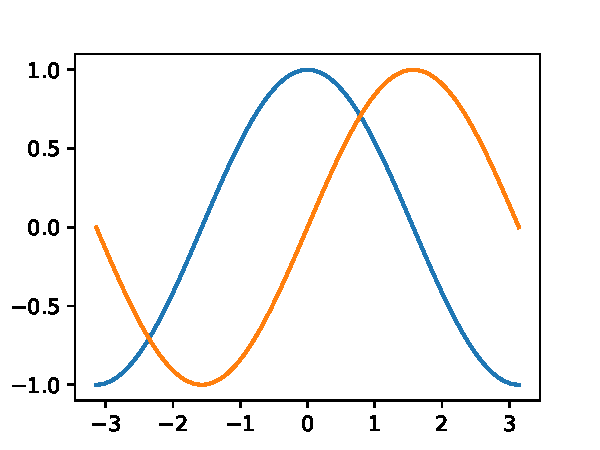
\includegraphics[width=10cm]{img/herramientas/grafico_sencillo}
	\caption{Gráfico simple en Matplotlib.}
	\label{fig:graficosencillo}
\end{figure}

\subsubsection{Modifiquemos este
gráfico}

Ahora, vamos a modificar algunos detalles de este gráfico.

\begin{listing}[H]
\begin{minted}[mathescape,
frame=lines,
framesep=2mm]{python}
# Creemos una figura de 6×4 in²
plt.figure(figsize=(6, 4))

# Usemos una línea solida,negra para el coseno de grosor 3
# y una línea punteada,roja para el coseno de grosor 1
plt.plot(x, cos, color="black", linestyle="solid", linewidth=2)
plt.plot(x, sin, color="red", linestyle="dashed", linewidth=1)

# Limitemos los ejes
plt.xlim(-4.0, 4.0)
plt.ylim(-1.5, 1.5)

# Asignemos nombre a cada eje
plt.xlabel("Eje x")
plt.ylabel("Eje y")

# Creemos una leyenda
plt.legend(["Coseno", "Seno"])

# Mostremos los resultados
plt.show()
\end{minted}
\end{listing}

\begin{figure}[H]
	\centering
	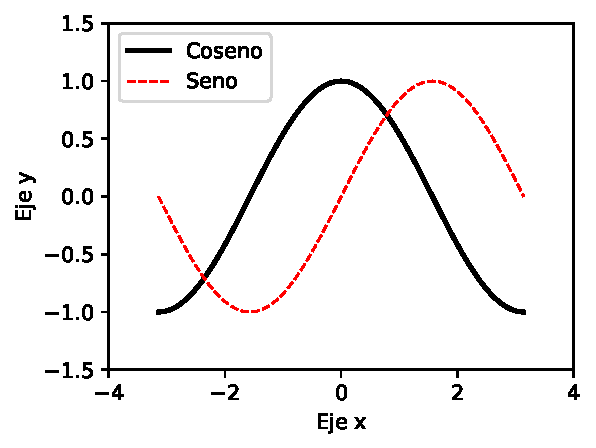
\includegraphics[width=10cm]{img/herramientas/grafico_sencillo_mejorado}
	\caption{Gráfico con configuración específica.}
	\label{fig:graficosencillo2}
\end{figure}

\subsection{Subplots}

Matplotlib nos permite organizar varios subgráficos (\texttt{axes}) en
una rejilla usando la función \texttt{subplot}.

\texttt{subplot} recibe como parámetros:

\begin{itemize}
\item
  Número de subgráficos (\texttt{axes}) en la dirección horizontal.
\item
  Número de subgráficos (\texttt{axes}) en la dirección vertical.
\item
  subgráfico (\texttt{axes}) actual.
\end{itemize}

Veamos un ejemplo

\begin{listing}[H]
\begin{minted}[mathescape,
frame=lines,
framesep=2mm]{python}
plt.figure(figsize=(8, 3))

# Usemos una rejila 2×1

# Primer subgráfico
plt.subplot(1, 2, 1)
plt.plot(x, cos)

# Segundo subgráfico
plt.subplot(1, 2, 2)
plt.plot(x, sin)

plt.show()
\end{minted}
\end{listing}

\begin{figure}[H]
	\centering
	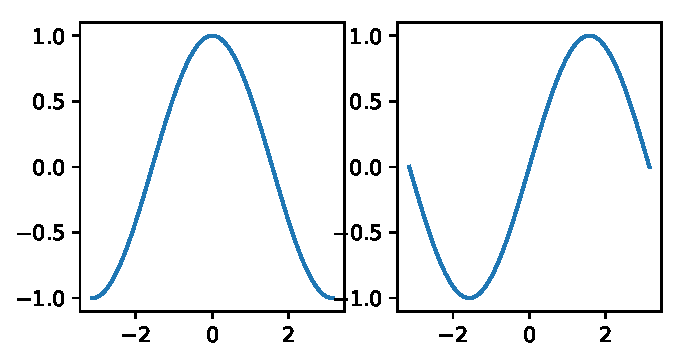
\includegraphics[width=10cm]{img/herramientas/subplots}
	\caption{Ejemplo de \emph{subplots}.}
	\label{fig:subplots}
\end{figure}

\subsection{Otros tipos de gráficos}

\subsubsection{Gráficos de dispersión}

Un gráfico de dispersión es un tipo de gráfico que utiliza coordenadas
cartesianas para mostrar los valores de dos variables para un conjunto
de datos. Los datos se presentan como una colección de puntos.

Mostremos un ejemplo con 1024 puntos aleatorios en el que el color de
cada punto dependa del ángulo.

\begin{listing}[H]
\begin{minted}[mathescape,
frame=lines,
framesep=2mm]{python}
# Definimos las coordenadas aleatoriamente
n = 1024
x = np.random.normal(0, 1, n)
y = np.random.normal(0, 1, n)

# Calculamos el ángulo usando  la función arcotangente
# que devuelve el ángulo en [-pi, pi]
angle = np.arctan2(y, x)

plt.figure(figsize=(4, 4))
plt.scatter(x, y, 20, angle, alpha=0.5)
\end{minted}
\end{listing}

\begin{figure}[H]
	\centering
	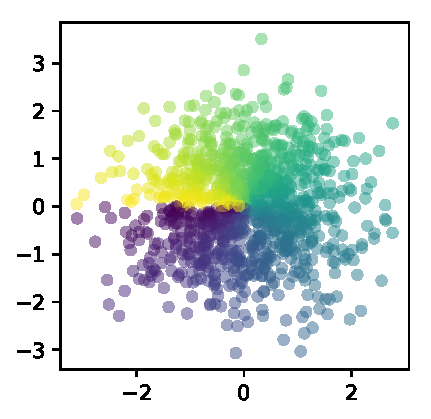
\includegraphics[width=8cm]{img/herramientas/grafico_dispersion}
	\caption{Ejemplo de gráfico de dispersión.}
	\label{fig:grafico_dispersion}
\end{figure}

\subsubsection{Gráfico de barras}

Un gráfico de barras usa barras rectangulares que son proprcionales a
los valores que representan. Uno de los ejes presenta las categorías que
se comparan, mientras el otro eje representa los valores.

Los gráficos de barras se utilizan en la presentación de datos
categóricos. Estos datos están agrupados en conjuntos discretos, como
meses del año, grupos de edad, o tamaños de zapatos.

Como ejemplo, grafiquemos los suicidios por edad en Colombia durante
2015. Los datos se obtuvieron de
\href{https://www.datos.gov.co/Estad-sticas-Nacionales/Suicidios-seg-n-Edad-/3nc9-zxcb/data}{www.datos.gov.co}.

\begin{listing}[H]
\begin{minted}[mathescape,
frame=lines,
framesep=2mm]{python}
edad = np.array(['80 y más', '75 a 79', '70 a 74', '65 a 69',
                 '60 a 64', '55 a 59', '50 a 54', '45 a 49',
                 '40 a 44', '35 a 39', '30 a 34', '25 a 29',
                 '20 a 24', '18 a 19', '15 a 17', '10 a 14'])
hombres = np.array([ 52,  33,  50,  62,  77, 99, 101, 134,
                    100, 145, 148, 191, 231, 95, 100,  37])
mujeres = np.array([ 6,  1,  4,  8, 13, 17, 22, 20, 19, 27,
                    41, 53, 71, 29, 49, 33])
\end{minted}
\end{listing}

Podemos usar la función \texttt{plt.bar} para realizar gráficos de
barras verticales y \texttt{plt.barh} para realizar gráficos de barras
horizontales.

El primer argumento se refiere a la posición (numérica) de cada dato. En
este caso, usaremos un número para cada valor, que podemos calcular
usando

\begin{listing}[H]
\begin{minted}[mathescape,
frame=lines,
framesep=2mm]{python}
posiciones = range(len(edad))
\end{minted}
\end{listing}

Mostraremos el ejemplo con barras horizontales, que permiten mejor leer
los rangos de edad en este caso.

\begin{listing}[H]
\begin{minted}[mathescape,
frame=lines,
framesep=2mm]{python}
plt.figure()
posiciones = range(len(edad))
# El parámetro opcional tick_label nos permite añadir cada rango
# de edades
plt.barh(posiciones, mujeres, tick_label=edad, color="#81bbea")
# Modificamos el alto de las barras para que no cubran las
# barras anteriores
plt.barh(posiciones, hombres, tick_label=edad, height=0.4,
         color="#377eb8")
plt.xlabel("Número de suicidios")
plt.ylabel("Edad")
plt.legend(["Mujeres", "Hombres"])
# El próximo comando obliga a Matplotlib a mostrar el
# gráfico completo
plt.tight_layout()
\end{minted}
\end{listing}

\begin{figure}[H]
	\centering
	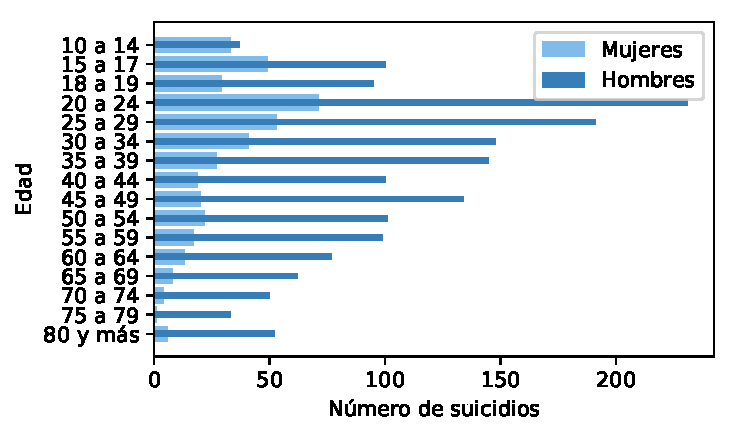
\includegraphics[width=13cm]{img/herramientas/grafico_barras}
	\caption{Ejemplo de gráfico de barras.}
	\label{fig:grafico_barras}
\end{figure}

\subsubsection{Gráfico de contornos}

Un gráfico de contornos permite representar la relación entre tres
variables numéricas en dos dimensiones. Dos de las variables representan
los ejes X e Y, y la tercera variable representa el nivel de os
contornos. Los contornos se grafican como curvas (\texttt{plt.contour});
el área entre las curvas de nivel puede colorearse como una
representación alternativa (\texttt{plt.contourf}).

Probemos con la siguiente función

\[f(x, y) = \left(1 - \frac{x}{2} + x^5 + y^3\right) e^{-x^2 - y^2}\]

\begin{listing}[H]
\begin{minted}[mathescape,
frame=lines,
framesep=2mm]{python}
def f(x, y):
    return (1 - x/2 + x**5 + y**3) * np.exp(-x**2 - y**2)
\end{minted}
\end{listing}

Este tipo de gráficos requiere que tengamos una rejilla, es decir, que
tengamos los pares \((x, y)\) para evaluar la función \(f(x, y)\). NumPy
nos permite hacer esto con la función \texttt{meshgrid}.

\begin{listing}[H]
\begin{minted}[mathescape,
frame=lines,
framesep=2mm]{python}
x = np.linspace(1, 5, 5)
y = np.linspace(1, 5, 5)
print("x:\textbackslash{n}", x)
print("y:\textbackslash{n}",y)

X, Y = np.meshgrid(x, y)
print("X:\textbackslash{n}", X)
print("Y:\textbackslash{n}", Y)
\end{minted}
\end{listing}

\begin{description}
\item[x:]
{[}1. 2. 3. 4. 5.{]}
\item[y:]
{[}1. 2. 3. 4. 5.{]}
\item[X:]
{[}{[}1. 2. 3. 4. 5.{]} {[}1. 2. 3. 4. 5.{]} {[}1. 2. 3. 4. 5.{]} {[}1.
2. 3. 4. 5.{]} {[}1. 2. 3. 4. 5.{]}{]}
\item[Y:]
{[}{[}1. 1. 1. 1. 1.{]} {[}2. 2. 2. 2. 2.{]} {[}3. 3. 3. 3. 3.{]} {[}4.
4. 4. 4. 4.{]} {[}5. 5. 5. 5. 5.{]}{]}
\end{description}

Veamos un ejemplo completo.

\begin{listing}[H]
\begin{minted}[mathescape,
frame=lines,
framesep=2mm]{python}
n = 256
# Creamos los valores de x e y en donde queremos evaluar la función
x = np.linspace(-3, 3, n)
y = np.linspace(-3, 3, n)

# Meshgrid los combina
X, Y = np.meshgrid(x, y)

plt.figure(figsize=(5, 5))
plt.contourf(X, Y, f(X, Y), 8, alpha=0.75, cmap="summer")
plt.contour(X, Y, f(X, Y), 8, colors='black')
\end{minted}
\end{listing}

\begin{figure}[H]
	\centering
	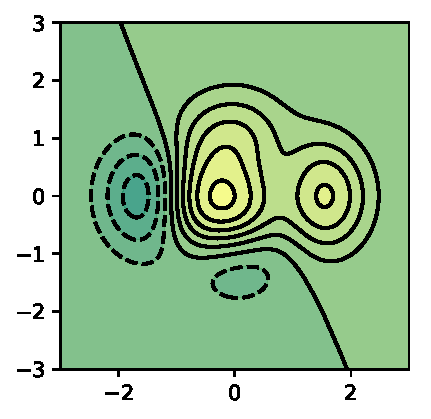
\includegraphics[width=8cm]{img/herramientas/grafico_contornos}
	\caption{Ejemplo de gráfico de contornos.}
	\label{fig:grafico_contornos}
\end{figure}

\subsubsection{Gráficos de campos vectoriales}

Presentamos dos métodos para graficar campos vectoriales. Uno de ellos
consiste en ubicar flechas con diferentes magnitudes y direcciones en
varios puntos del espacio y la otra usa líneas de corriente

\begin{listing}[H]
\begin{minted}[mathescape,
frame=lines,
framesep=2mm]{python}
x = np.linspace(-2, 1, 21)
y = np.linspace(-2, 2, 21)
X, Y = np.meshgrid(x, y)
U = Y
V = -X - X**2

plt.figure()
plt.quiver(X, Y, U, V)
\end{minted}
\end{listing}

\begin{figure}[H]
	\centering
	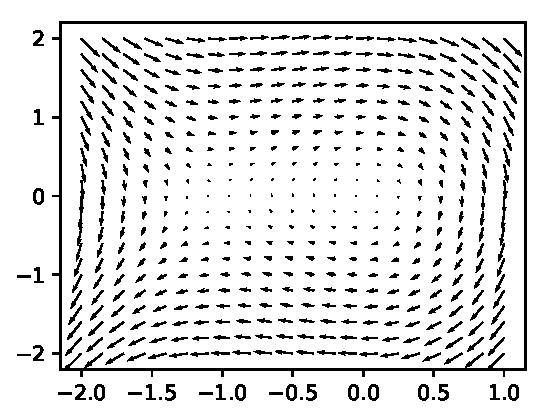
\includegraphics[width=10cm]{img/herramientas/grafico_flechas}
	\caption{Ejemplo de gráfico de campo vectorial usando flechas.}
	\label{fig:grafico_flechas}
\end{figure}

\begin{listing}[H]
\begin{minted}[mathescape,
frame=lines,
framesep=2mm]{python}
x = np.linspace(-2, 1, 21)
y = np.linspace(-2, 2, 21)
X, Y = np.meshgrid(x, y)
U = Y
V = -X - X**2

plt.figure()
plt.streamplot(X, Y, U, V)
\end{minted}
\end{listing}

\begin{figure}[H]
	\centering
	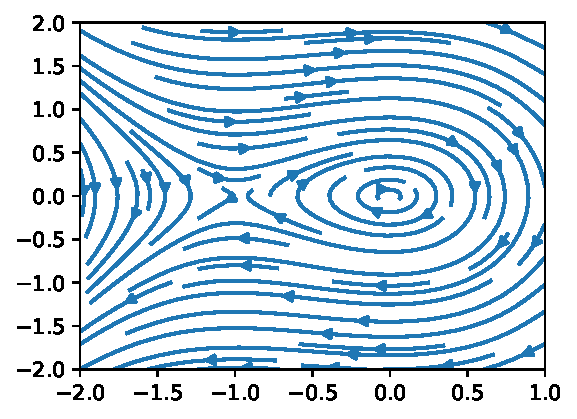
\includegraphics[width=10cm]{img/herramientas/grafico_lineas_corriente}
	\caption{Ejemplo de gráfico de campo vectorial usando lineas de corriente.}
	\label{fig:grafico_lineas_corriente}
\end{figure}

\subsubsection{Gráficos 3D}

Matplotlib ofrece la capacidad de realizar gráficos 3D usando el módulo
\texttt{mpl\_toolkits.mplot3d}. Para hacer uso de este debemos realizar
su importación como se muestra a continuación.

\begin{listing}[H]
\begin{minted}[mathescape,
frame=lines,
framesep=2mm]{python}
from mpl_toolkits.mplot3d import Axes3D
\end{minted}
\end{listing}

\begin{listing}[H]
\begin{minted}[mathescape,
frame=lines,
framesep=2mm]{python}
n = 51
x = np.linspace(-3, 3, n)
y = np.linspace(-3, 3, n)
X, Y = np.meshgrid(x, y)

fig = plt.figure()
# Luego de crear la figura, creamos un contenedor (Axes3D)
ax = Axes3D(fig)
ax.plot_surface(X, Y, f(X,Y), cmap="viridis")
\end{minted}
\end{listing}

\begin{figure}[H]
	\centering
	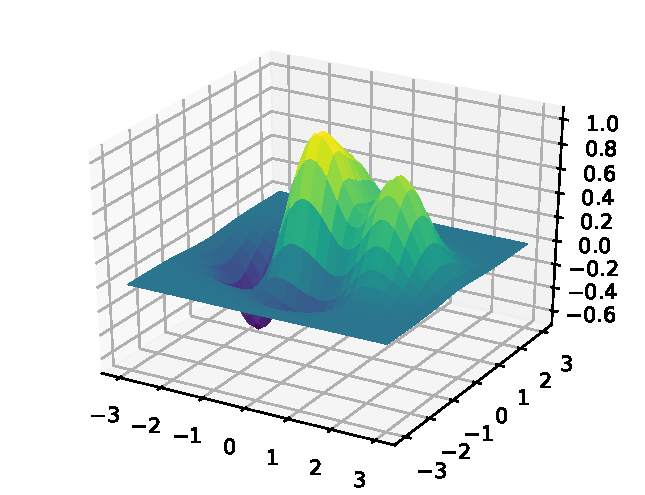
\includegraphics[width=10cm]{img/herramientas/grafico_superficie}
	\caption{Ejemplo de gráfico de superficie.}
	\label{fig:grafico_superficie}
\end{figure}

\begin{listing}[H]
\begin{minted}[mathescape,
frame=lines,
framesep=2mm]{python}
fig = plt.figure()
ax = Axes3D(fig)
ax.contour(X, Y, f(X,Y), 20)
\end{minted}
\end{listing}

\begin{figure}[H]
	\centering
	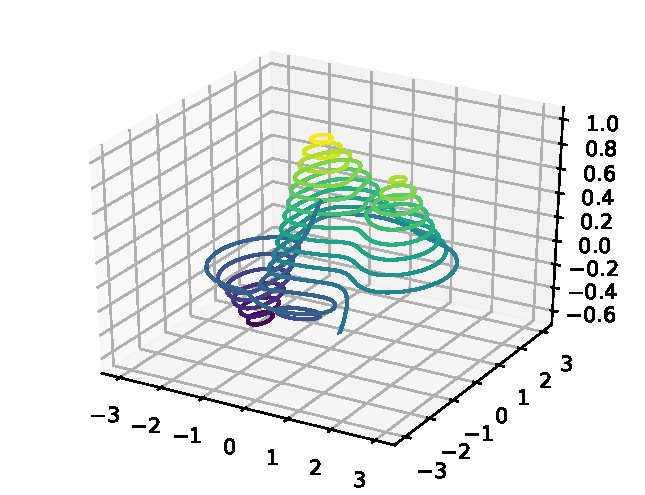
\includegraphics[width=10cm]{img/herramientas/grafico_contorno3D}
	\caption{Ejemplo de gráfico de contornos 3D.}
	\label{fig:grafico_contorno3D}
\end{figure}

\begin{listing}[H]
\begin{minted}[mathescape,
frame=lines,
framesep=2mm]{python}
fig = plt.figure()
ax = Axes3D(fig)
ax.contourf(X, Y, f(X,Y), 20)
\end{minted}
\end{listing}

\begin{figure}[H]
	\centering
	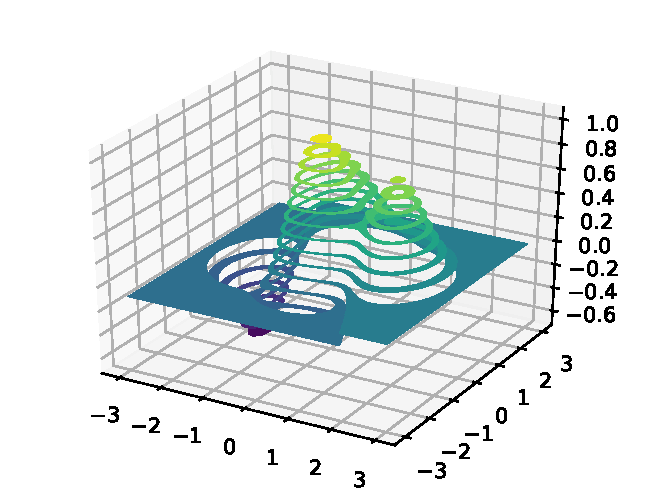
\includegraphics[width=10cm]{img/herramientas/grafico_contorno_lleno_3D}
	\caption{Ejemplo de gráfico de contornos 3D.}
	\label{fig:grafico_contorno_lleno_3D}
\end{figure}

\subsection{Actividad}

Se desea obtener el siguiente gráfico

\begin{figure}[H]
    \centering
    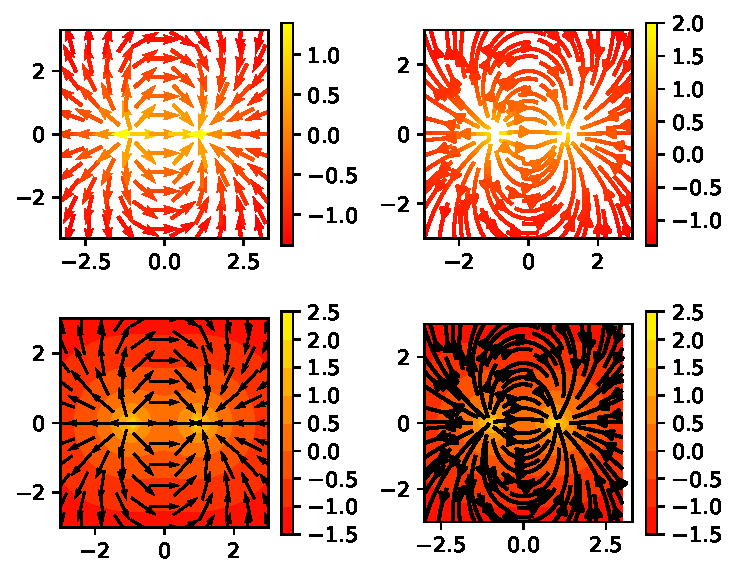
\includegraphics[width=13cm]{campo_electrico}
\end{figure}

en donde se está graficando:

\begin{enumerate}
\def\labelenumi{\arabic{enumi}.}

\item
  El campo eléctrico (campo vectorial) dado por
\end{enumerate}

\[\mathbf{E} = \sum_{i=1}^2 q_i \frac{\mathbf{r} - \mathbf{r}_i}{\Vert \mathbf{r}\Vert^3}\, .\]

\begin{enumerate}
\def\labelenumi{\arabic{enumi}.}
\setcounter{enumi}{1}

\item
  La magnitud del campo eléctrico (campo escalar) como mapa de colores.
\end{enumerate}

Las posiciones de las partículas son: \((-1, 0)\) y \((1, 0)\). Sus
cargas son \(q_1 = 1\) y \(q_2=-1\).

\subsection{Recursos adicionales}

\begin{enumerate}
\def\labelenumi{\arabic{enumi}.}

\item
  Nicolas Rougier, Mike Müller, Gaël Varoquaux.
  \href{http://www.scipy-lectures.org/intro/matplotlib/index.html}{Matplotlib:
  plotting}, 2018.
\item
  Equipo de desarrollo de Matplotlib.
  \href{https://matplotlib.org/gallery/index.html}{Galería}, 2018.
\end{enumerate}


\section{Interfaces gráficas}

El papel del desarrollo de interfaces gráficas en la modelación es facilitar la
creación del flujo de trabajo con un código, como la selección de archivos, la
configuración de parámetros o la presentación de resultados. En particular, facilitará
el acercamiento al programa desarrollado para personas que no tienen conocimiento técnico.

Una interfaz gráfica puede tener desventajas también, como lo es un mayor consumo de
memoria en comparación a una interfaz no gráfica (cliente de comandos), toma mayor tiempo
de desarrollo y un mal diseño puede dificultar su manejo.

Existen distintas bibliotecas para el diseño de interfaces gráficas que puedan
usarse con Python, cada una con sus ventajas y desventajas, pero para este curso
nos enfocaremos solo en una aunque mencionaremos brevemente algunas opciones multiplataforma
(disponibles en Windows, Mac y Linux).

\begin{itemize}
    \item[Qt5] Es un \textit{framework} C++ donde los elementos gráficos son emulados
    usando OpenGL (no son controles nativos y su apariencia no depende del sistema operativo)
    y disponible en Python a través de los proyectos PyQt5 y PySide. Es de fácil instalación
    en los tres sistemas operativos mencionados.
    \item[WxWidgets] Es otro \textit{framework} C++ que a diferencia de Qt si usa controles
    nativos (lo cual mejora el rendimiento de la interfaz). Está disponible en Python a través del
    proyecto WxPython Phoenix.
    \item[Tk] Es la biblioteca gráfica desarrollada para el lenguaje Tcl y disponible en la instalación
    de Python en su núcleo (implementación oficial, CPython).
    \item[Kivy] Es un \textit{framework} Python optimizado con Cython que usa controles nativos.
    \item[Toga] Es una biblioteca gráfica en Python puro que invoca directamente a los controles nativos,
    lo cual hace bastante eficiente la interfaz gráfica y fácil de instalar.
    \item[GTK] Disponible en Python a través del proyecto PyGTK y PyGObject (este último reemplazo a PyGTK).
    \item[Jupyter] El proyecto Jupyter dispone de los Jupyter Widgets para integrar con los Notebooks. Son
    controles javascript para la interfaz interactiva del documento web. No solo son multiplataforma sino que
    también están disponibles para las versiones de documento web de otros lenguajes.
    \item[easyGUI] Es una biblioteca de controles gráficos pensada en un uso fácil. Esta es la herramienta
    que recomendamos en el curso.
\end{itemize}

\subsection{Instalación}

El proceso de instalación de easyGUI se hace a través de la consola de Anaconda (\textit{Anaconda Prompt}) a través de la siguiente
instrucción.

\begin{listing}[H]
    \begin{minted}[mathescape, gobble=8, frame=lines,
            framesep=2mm]{bash}
        pip install easygui
    \end{minted}
\end{listing}

\subsection{Uso básico}

EasyGUI define un rápido acceso a los elementos de interacción, siendo bastante simple crear los primeros controles
para un programa en pocas líneas. Se sacrifica el nivel de personalización para reducir el código pero de requerirlo
EasyGUI también permite interfaces más elaboradas.

Para invocar el módulo procedemos como:

\begin{listing}[H]
    \begin{minted}[mathescape, gobble=8, frame=lines,
            framesep=2mm]{python}
        import easygui
    \end{minted}
\end{listing}

Podemos crear un control de aceptación (marco con dos botones que generan el valor de falso o verdadero)
con el bloque de código dado en \ref{lst:confirmar} y se ve como ilustra la figura
\ref{fig:ynbox}.

\begin{listing}[H]
    \begin{minted}[mathescape, gobble=8, frame=lines,
            framesep=2mm]{python}
        easygui.ynbox("Confirmar matrícula", "Matrícula", ("Aceptar", "Negar"))
    \end{minted}
    \caption{Código para un bloque de confirmación.}
    \label{lst:confirmar}
\end{listing}

\begin{figure}
    \centering
    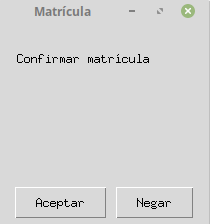
\includegraphics[height = 3 in]{ynbox.png}
    \caption{Control de aceptación con EasyGUI en Linux.}
    \label{fig:ynbox}
\end{figure}

También es posible crear mensajes de alerta con el código \ref{lst:alerta} y se observa como la
figura \ref{fig:msgbox}.

\begin{listing}[H]
    \begin{minted}[mathescape, gobble=8, frame=lines,
            framesep=2mm]{python}
        easygui.msgbox("Ha terminado la ejecución", "Simulación")
    \end{minted}
    \caption{Bloque de código para crear un mensaje de alerta.}
    \label{lst:alerta}
\end{listing}

\begin{figure}
    \centering
    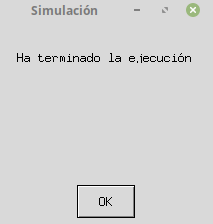
\includegraphics[height = 3 in]{msgbox.png}
    \caption{Mensaje de alerta con EasyGUI en Linux.}
    \label{fig:msgbox}
\end{figure}

Se pueden crear botones como con el código \ref{lst:boton} y obtener el cuadro mostrado en \ref{fig:buttonbox}.

\begin{listing}[H]
    \begin{minted}[mathescape, gobble=8, frame=lines,
            framesep=2mm]{python}
        easygui.buttonbox("Tarea a entregar", "Tareas", ("1", "2", "3"))
    \end{minted}
    \caption{Control de botones con EasyGUI en Linux.}
    \label{lst:boton}
\end{listing}

\begin{figure}
    \centering
    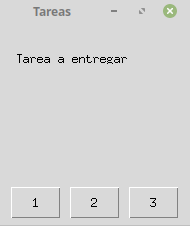
\includegraphics[height = 3 in]{buttonbox.png}
    \caption{Control con botones con EasyGUI en linux.}
    \label{fig:buttonbox}
\end{figure}

Igualmente existen muchos más controles de utilidad, como los son controles para la exploración
de archivos y directorios.

Para saber más, puede referirse al tutorial disponible en la documentación oficial del paquete,
\href{http://easygui.sourceforge.net/tutorial.html}{EasyGui Tutorial}.

\subsection{Actividad}

Realice una rutina que permita la selección gráfica de dos archivos CSV. El primer archivo contiene
los datos de una matriz cuadrada \(A\) y el segundo archivo los datos de un vector \(b\). El código debe permitir
seleccionar gráficamente el destino del archivo de salida que contendrá la solución del sistema \(Ax=b\). En caso
del sistema no tener solución se debe generar un mensaje de alerta indicando el error. Personalice el mensaje de
error al menos para los siguientes casos:

\begin{enumerate}
\item La matriz \(A\) no es cuadrada.
\item Las dimensiones de \(A\) y \(b\) no son consistentes.
\item Archivo vacío.
\item No se ha encontrado solución.
\end{enumerate}

